\begin{addendum}
(Construcción explícita de las curvas del ejercicio 2.b)
\end{addendum}

\begin{solution}
Para construir las curvas rojas, variemos $t$ desde $0$ hasta $2\pi$. Para construir las curvas azules, variemos $t$ desde $0$ hasta $-2\pi$. Las curvas en el plano $\C_3$ son arcos circulares descritos por $w = e^{it/3}$:
\begin{figure}[h]
    \centering
    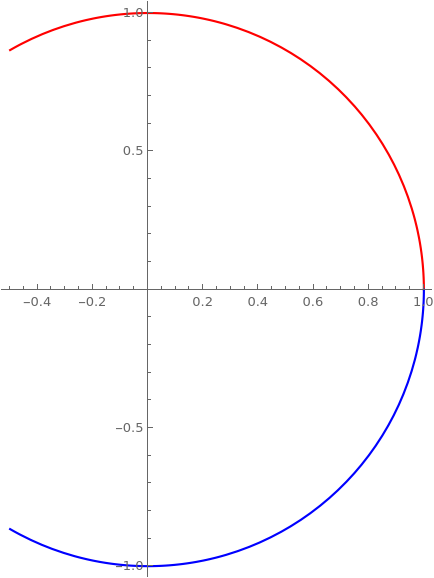
\includegraphics[scale=0.4]{c3.png}
    \caption{Una vecindad del origen en $\C_3$.}
\end{figure}

\newpage

Ambas curvas se proyectan a $\C_1$ como el círculo $z^2 = e^{it} - 1$:
\begin{figure}[h]
    \centering
    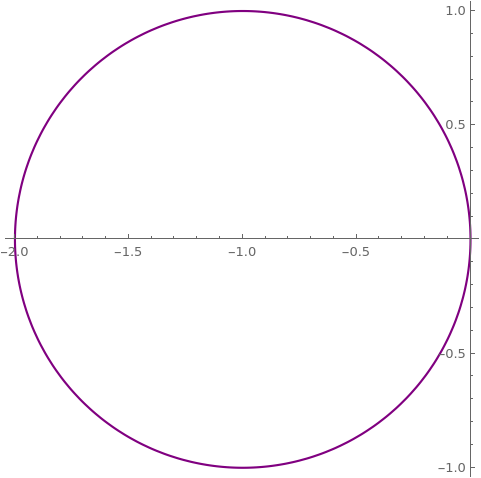
\includegraphics[scale=0.4]{c1.png}
    \caption{Una vecindad del punto $z^2 = -1$ en $\C_1$.}
\end{figure}

Escribamos la coordenada de $\C_2$ como $z = re^{i\theta}$. Entonces,
$$r^4 = |z^2|^2 = (1 - \cos t)^2 + (\sin t)^2 = 2 - 2 \cos t$$
$$\cos^2 2\theta
    = \frac {(1 - \cos t)^2} {2 - 2 \cos t}
    = \frac {1 - \cos t} 2
    = \frac {r^4} 4
$$

Notemos que $\cos 2\theta \le 0$, porque $\Im(z^2) \le 0$. Entonces la ecuación de las curvas en $\C_2$ es
$$r^2 = -2 \cos 2\theta$$

Recordemos que no hay ambigüedad sobre el signo de $r$: en coordenadas polares, siempre $r > 0$. Para dibujar la curva roja en $\C_2$, haremos variar $\theta$ desde $\pi/4$ hasta $3\pi/4$. Para dibujar la curva azul, haremos variar $\theta$ desde $-\pi/4$ hasta $-3\pi/4$. Obtenemos el siguiente resultado:
\begin{figure}[h]
    \centering
    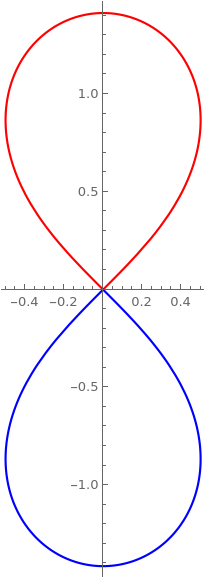
\includegraphics[scale=0.5]{c2.png}
    \caption{Las curvas buscadas en $\C_2$.}
\end{figure}
\end{solution}
